\section{Activity Distribution}

To asses the amount of the test population that accounted for similar types of activation patterns, an activity distribution analysis was carried out. The analysis was carried out by assessing the patterns of activation in population subsets of 10-30$\percent$, 40-60$\percent$ and 70-100$\percent$. The preprocessing method resulting in the smallest size of activation was superimposed on the larger to illustrate differences.  

\Figref{fig:10} illustrates the activation that was common across 10-30$\percent$ of the test population. Large areas of activation were common after the use of both methods. Differences were found in the brain stem, where both positive and negative activation seem to have been reduced after the use of FIX. This might indicate that a reduction in physiological noise has been achieved when assessing what was common activation for 10-30$\percent$ of the test population. Using FIX has also resulted in an increase of negative activation in the inferior edge of the cerebellum. This activation should be considered as noise in the task-related design used in this project.

\begin{figure}[H]%
	\centering
	\subfigure[Positive activation map]{%
		\label{fig:first}%
		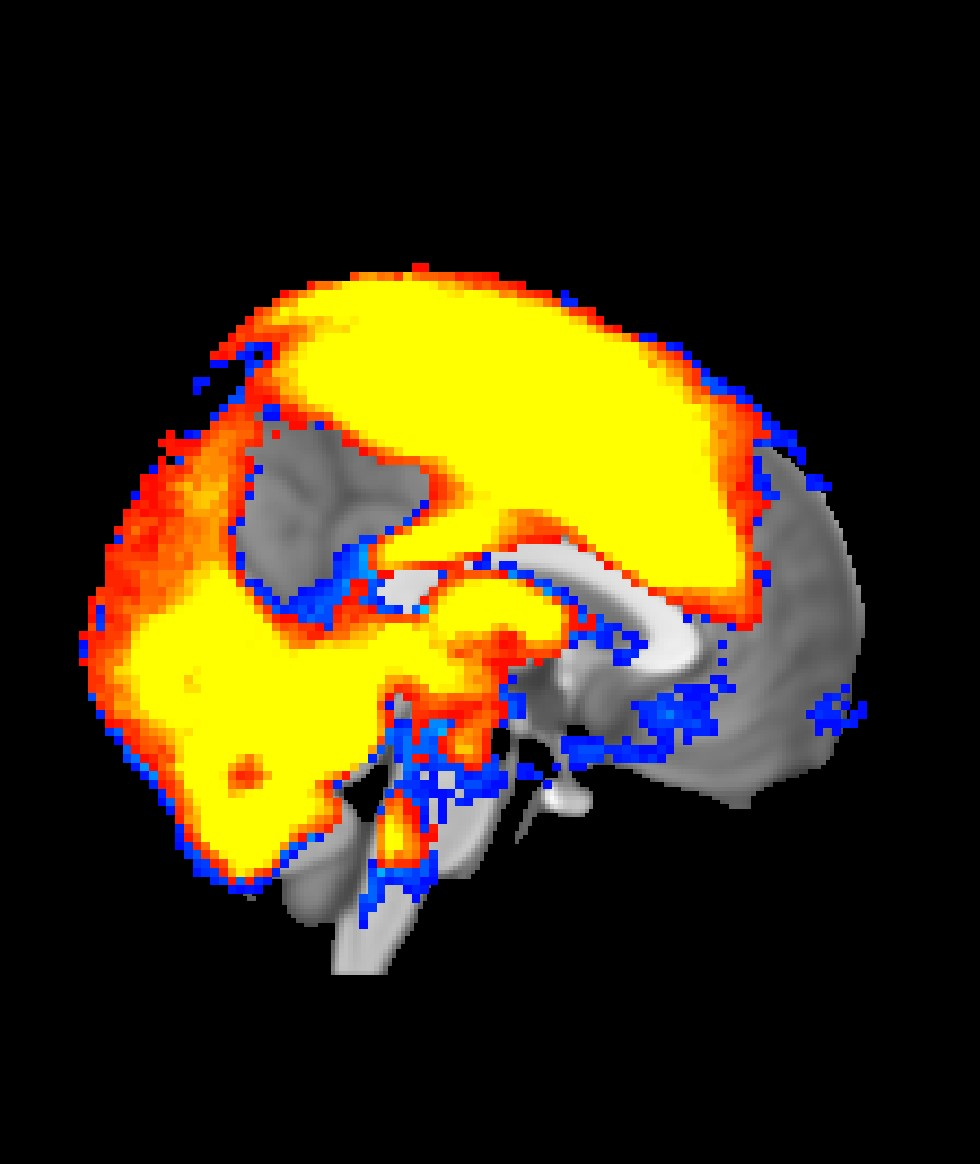
\includegraphics[width=.42\textwidth]{figures/Results/Pos_10-30}}%
	\qquad
	\subfigure[Negative activation map]{%
		\label{fig:second}%
		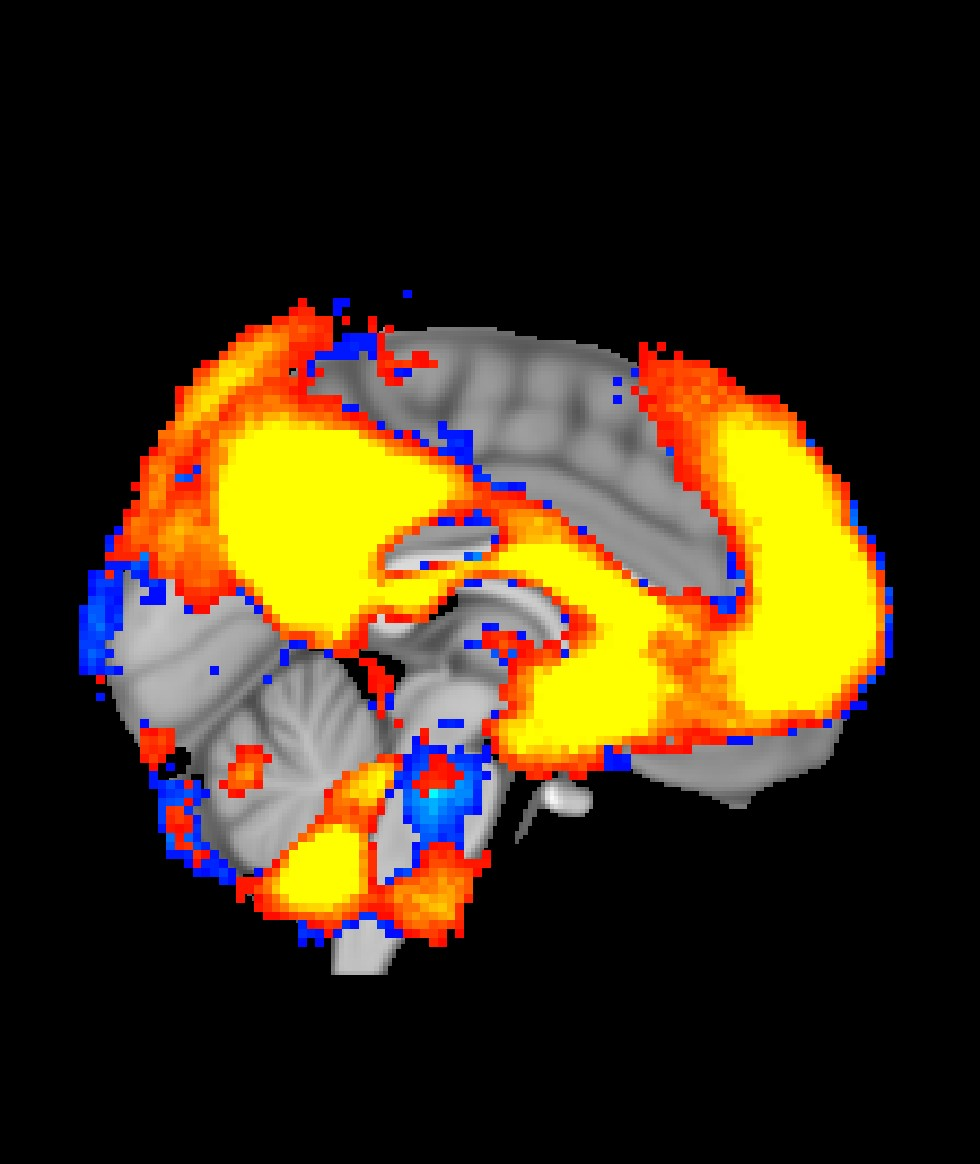
\includegraphics[width=.42\textwidth]{figures/Results/Neg_10-30}}%
	\caption{Positive activation (a) and negative activation (b) common for 10-30$\percent$ of the test population. Blue is the activation after using standard preprocessing and red is after using FIX preprocessing. FIX preprocessing is superimposed on the activation achieved using the standard preprocessing illustrating differences in activation between the methods.}
	\label{fig:10}
\end{figure}

Increasing the amount of the test population from which activation was common for 40-60$\percent$ of the population did not show any greater differences in activation between standard preprocessing and FIX as illustrated in \figref{fig:40}. In the positive map similar activation is seen in both the anterior cingulate cortex and cerebellum, and similar area size of deactivation is seen in the posterior cingulate cortex. Using FIX for preprocessing increased the prefrontal deactivation compared to standard preprocessing as seen in the negative map. Finally, FIX resulted in an increased deactivation in a part of the subcollosal gyrus area.

\begin{figure}[H]%
	\centering
	\subfigure[Positive activation map]{%
		\label{fig:first}%
		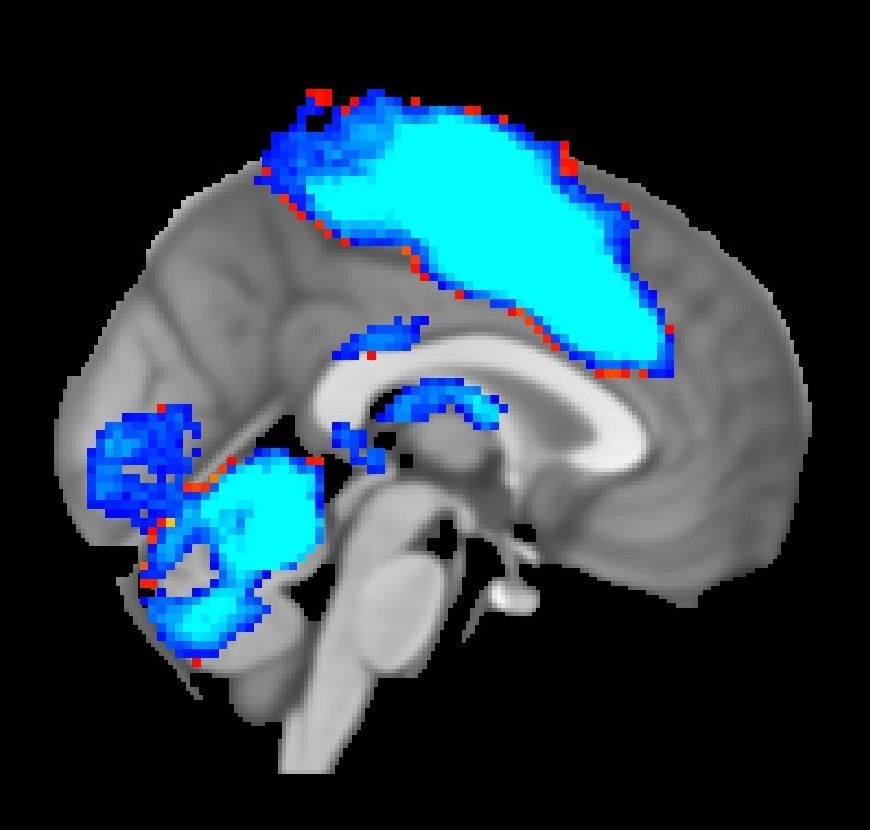
\includegraphics[width=.42\textwidth]{figures/Results/Pos_40-60}}%
	\qquad
	\subfigure[Negative activation map ]{%
		\label{fig:second}%
		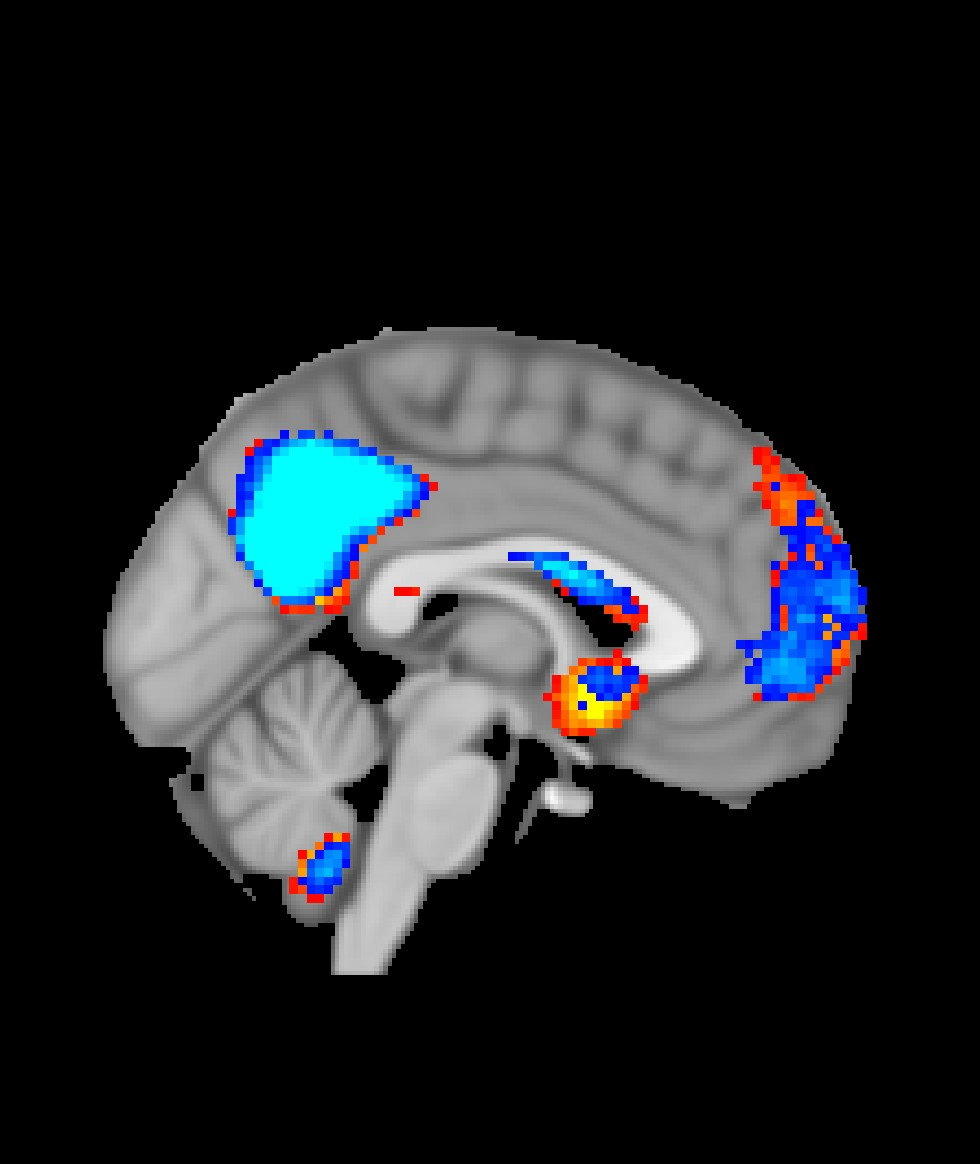
\includegraphics[width=.42\textwidth]{figures/Results/Neg_40-60}}%
	\caption{Positive activation (a) and negative activation (b) common for 40-60$\percent$ of the test population. Blue is the activation after using standard preprocessing and red is after using FIX preprocessing. Activation achieved using the standard preprocessing is superimposed on activation achieved using the FIX preprocessing illustrating differences in activation between the methods.}
	\label{fig:40}
\end{figure}

Increasing the amount of the test population from which activation was common for >70$\%$ of the population further limited the areas of activation as seen on \figref{fig:70}. In the positive map the area of activation in the anterior cingulate cortex is larger when using FIX illustrating a higher amount signal of interest preserved. In the negative map only 92$\percent$ of the participant had the similar deactivation of the posterior cingulate cortex, indicating that activation in this area is not common for all participants. 

\begin{figure}[H]%
	\centering
	\subfigure[Positive activation map]{%
		\label{fig:first}%
		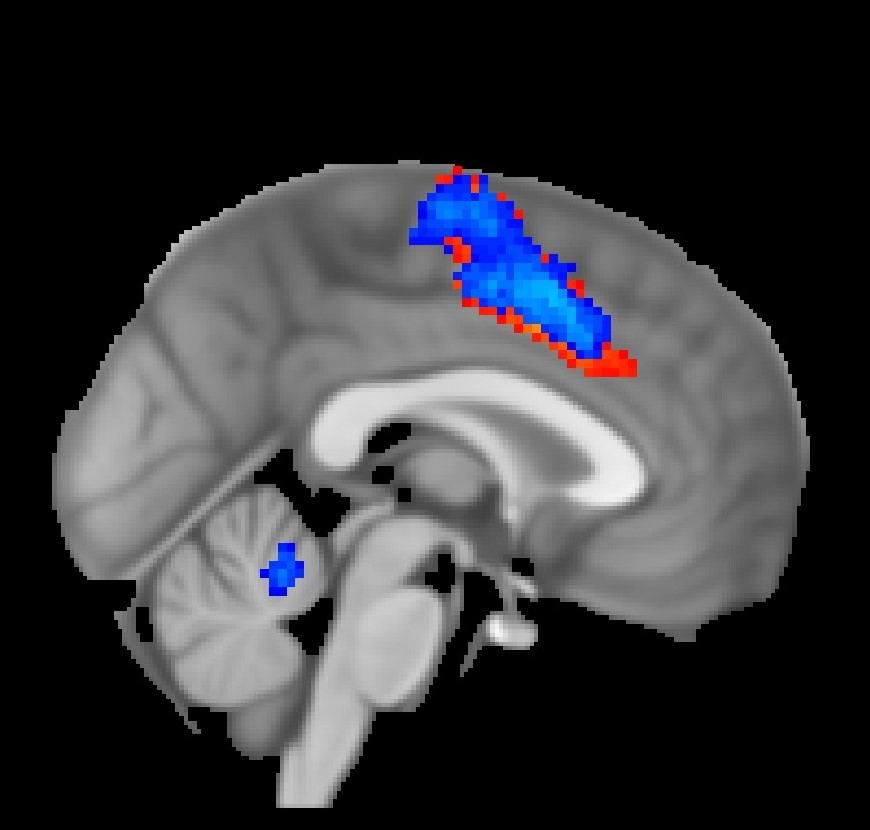
\includegraphics[width=.42\textwidth]{figures/Results/Pos_80-100}}%
	\qquad
	\subfigure[Negative activation map]{%
		\label{fig:second}%
		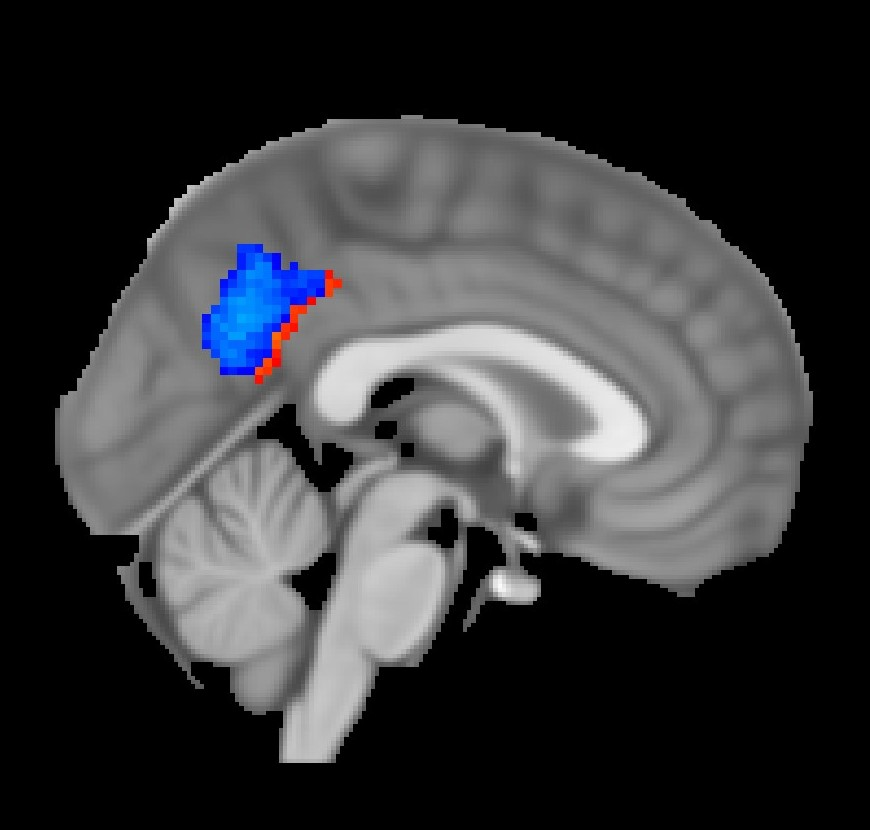
\includegraphics[width=.42\textwidth]{figures/Results/Neg_70-92}}%
	\caption{Positive activation (a) and negative activation (b) common for 80-100$\percent$ of the test population in the positive map and 70-92$\percent$ in the negative map. Blue is the activation after using standard preprocessing and red is after using FIX preprocessing. Activation achieved using the standard preprocessing is superimposed on the activation achieved using FIX preprocessing illustrating differences in activation between the methods.}
	\label{fig:70}
\end{figure}


%\begin{figure}[H]                 
%	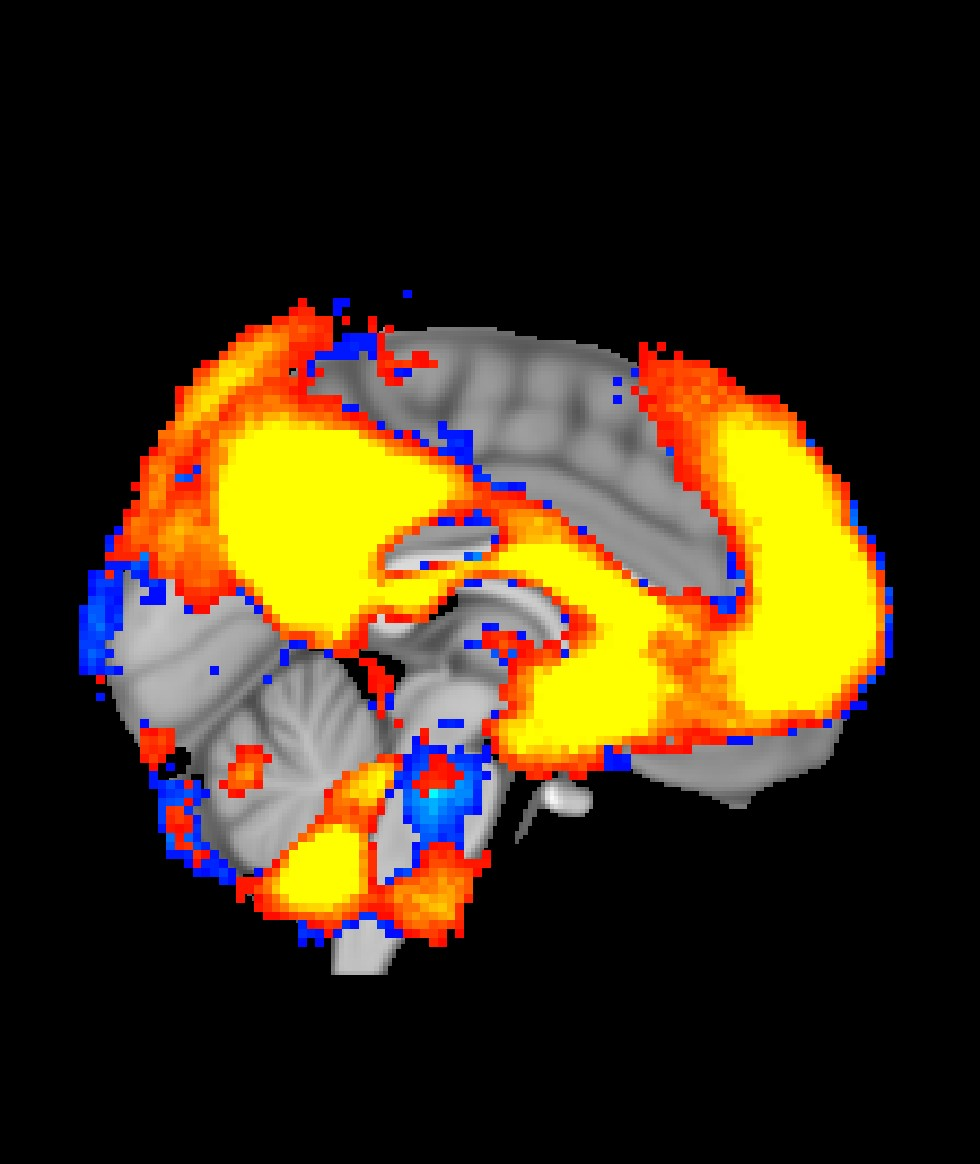
\includegraphics[width=.45\textwidth]{figures/Results/Neg_10-30}  
%	\caption{An example component of signal, which is recognizable, isolated, and not corrupted by a substantial amount of noise. In this example, the signal is characterized as a strong and fairly isolated activation mainly in the parietal lobe and some in the temporal lobe.}
%	\label{fig:res:diffpos} 
%\end{figure}
%
%\begin{figure}[H]                 
%	\includegraphics[width=.45\textwidth]{}  
%	\caption{An example component of signal, which is recognizable, isolated, and not corrupted by a substantial amount of noise. In this example, the signal is characterized as a strong and fairly isolated activation mainly in the parietal lobe and some in the temporal lobe.}
%	\label{fig:res:diffneg} 
%\end{figure}
%
%\begin{figure}[H]                 
%	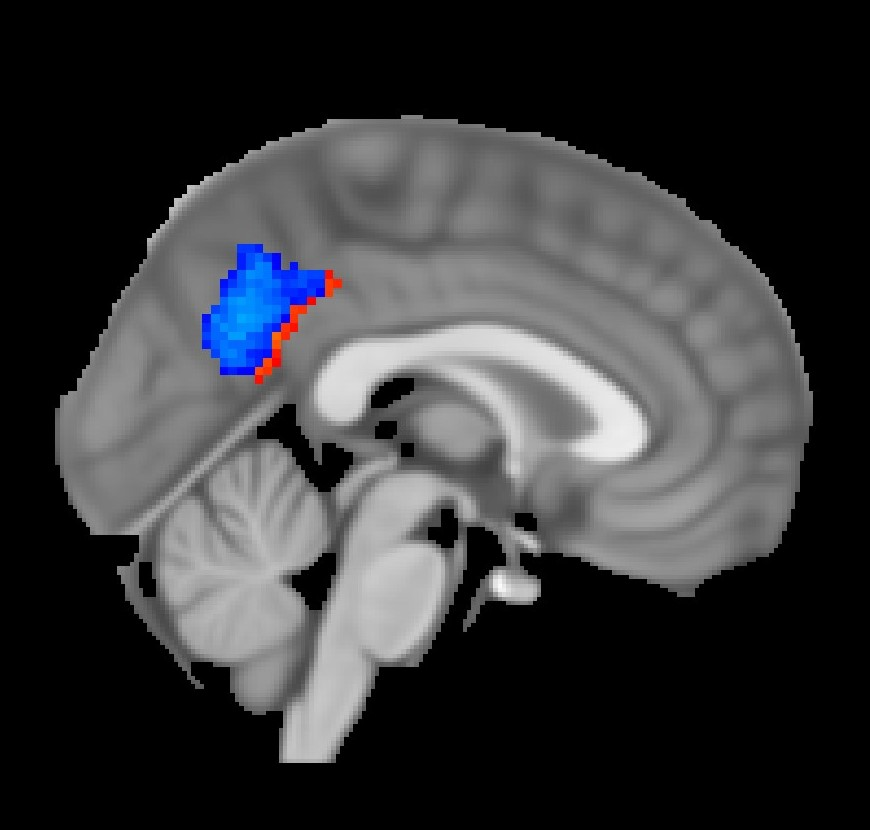
\includegraphics[width=.65\textwidth]{figures/Results/Neg_70-92}  
%	\caption{An example component of signal, which is recognizable, isolated, and not corrupted by a substantial amount of noise. In this example, the signal is characterized as a strong and fairly isolated activation mainly in the parietal lobe and some in the temporal lobe.}
%	\label{fig:res:diffneg} 
%\end{figure}
%
%\begin{figure}[H]                 
%	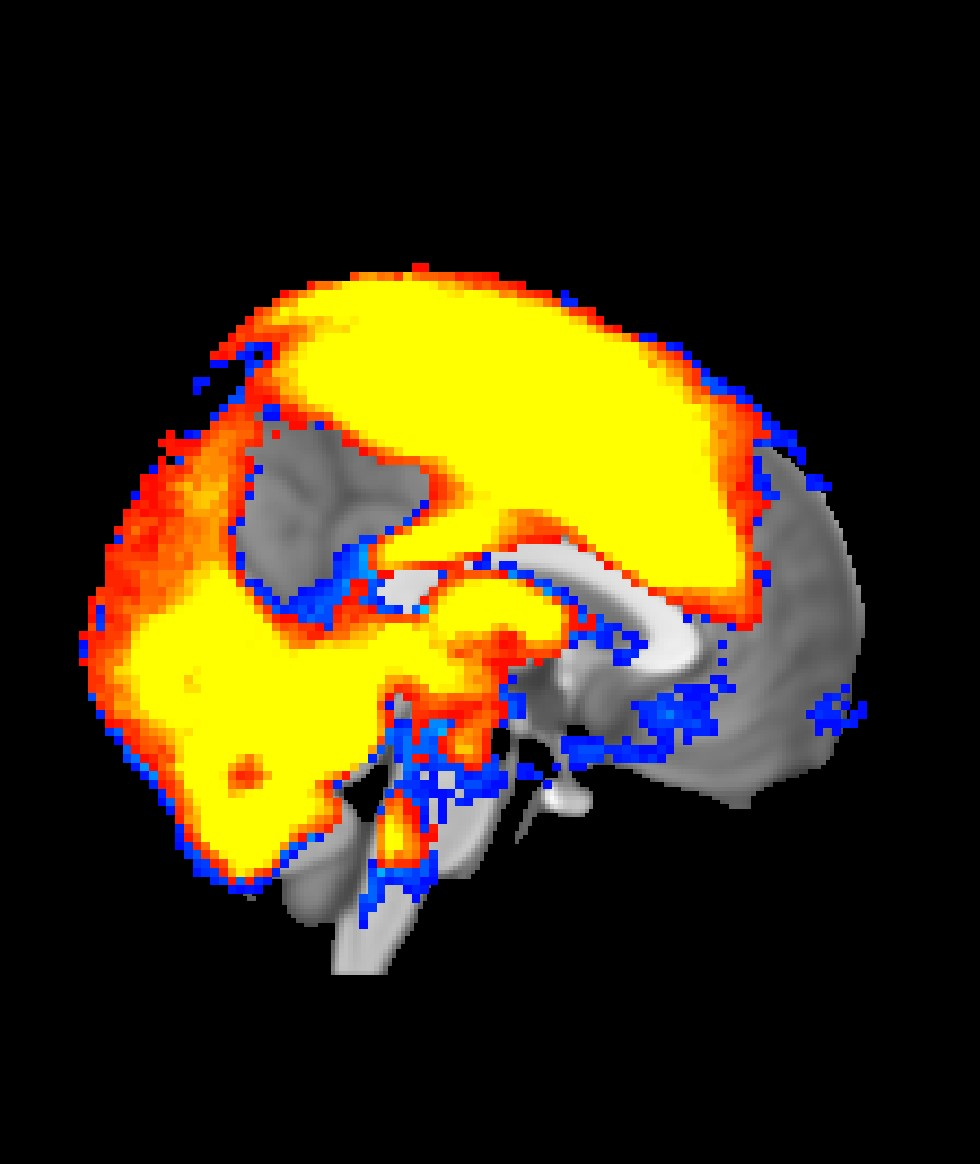
\includegraphics[width=.65\textwidth]{figures/Results/Pos_10-30}  
%	\caption{An example component of signal, which is recognizable, isolated, and not corrupted by a substantial amount of noise. In this example, the signal is characterized as a strong and fairly isolated activation mainly in the parietal lobe and some in the temporal lobe.}
%	\label{fig:res:diffpos} 
%\end{figure}
%
%\begin{figure}[H]                 
%	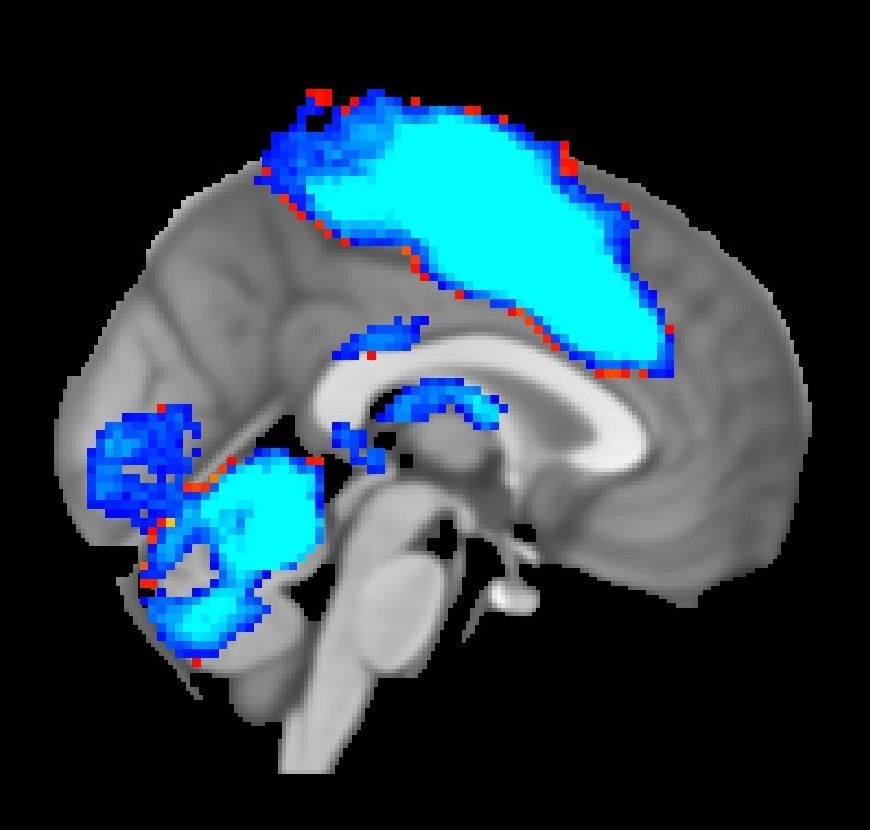
\includegraphics[width=.65\textwidth]{figures/Results/Pos_40-60}  
%	\caption{An example component of signal, which is recognizable, isolated, and not corrupted by a substantial amount of noise. In this example, the signal is characterized as a strong and fairly isolated activation mainly in the parietal lobe and some in the temporal lobe.}
%	\label{fig:res:diffneg} 
%\end{figure}
%
%\begin{figure}[H]                 
%	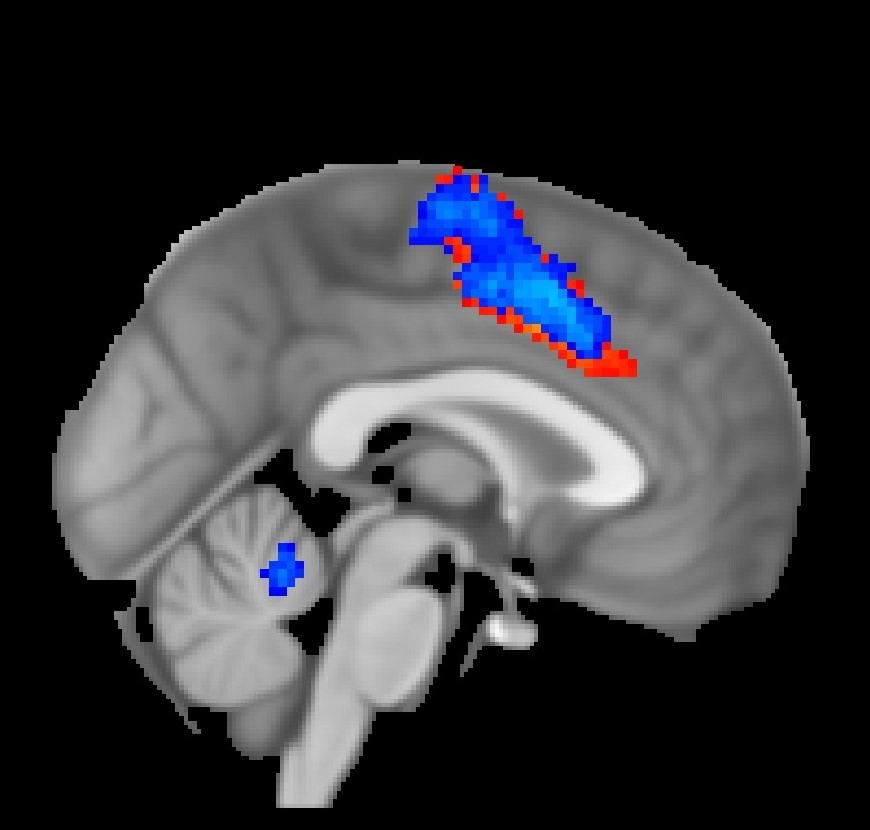
\includegraphics[width=.65\textwidth]{figures/Results/Pos_80-100}  
%	\caption{An example component of signal, which is recognizable, isolated, and not corrupted by a substantial amount of noise. In this example, the signal is characterized as a strong and fairly isolated activation mainly in the parietal lobe and some in the temporal lobe.}
%	\label{fig:res:diffneg} 
%\end{figure}